\documentclass{standalone}
\usepackage{tikz}
\begin{document}
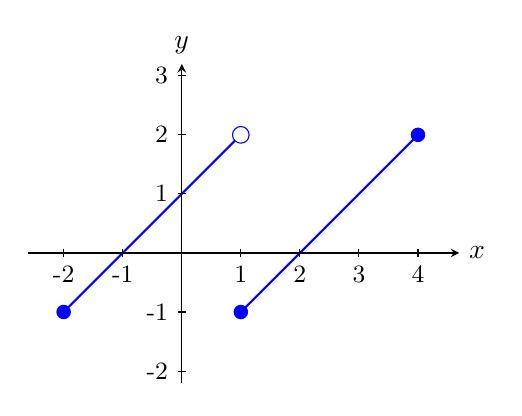
\begin{tikzpicture}[>=stealth, scale=0.75]
  % Jump discontinuity at x = 1:
  % left piece:  y = x + 1 on [-2, 1), open circle at (1, 2)
  % right piece: y = x - 2 on [1, 4], filled dot at (1, -1)
  \draw[blue, thick] (-2,-1) -- (1,2);
  \draw[blue, thick] (1,-1) -- (4,2);
  % Axes
  \draw[->] (-2.6,0) -- (4.7,0) node[right] {$x$};
  \draw[->] (0,-2.2) -- (0,3.2) node[above] {$y$};
  % x-axis ticks
  \foreach \x in {-2,-1,1,2,3,4} {
    \draw (\x,0.07) -- (\x,-0.07) node[below, font=\small] {\x};
  }
  % y-axis ticks
  \foreach \y in {-2,-1,1,2,3} {
    \draw (0.07,\y) -- (-0.07,\y) node[left, font=\small] {\y};
  }
  % Endpoints of the domain
  \fill[blue] (-2,-1) circle (3.5pt);
  \fill[blue] (4,2) circle (3.5pt);
  % Open circle at (1,2) -- left-hand limit
  \draw[fill=white, draw=blue] (1,2) circle (4pt);
  % Filled dot at (1,-1) -- f(1) = -1
  \fill[blue] (1,-1) circle (3.5pt);
\end{tikzpicture}
\end{document}
